\chapter{无人机集群行为数据的分布漂移检测方法研究}
\label{chapter:swarm-distributions}

\section{引言}
\label{Introduction}
根据第\ref{chap:edbed}章关于机器学习一致收敛的理论分析可知, 机器学习算法的基本前提假设是经验数据由固定的、但是未知的分布独立地生成\citep{vapnik1995, vapnik1998, Vapnik2006}。 在具体实际应用中, 研究者通常会将得到的数据集随机采样为训练集和测试集。根据Bruno de Finetti(1906-1985)提出的现代概率论批判理论\citep{Finetti1975}, 将经验数据利用现代计算技术随机处理后能使得经验数据满足概率论理论要求, 但同时也将经验数据本身的分布信息忽视\citep{shiryaev2016-1,shiryaev2016-2}。

在开展有关无人机集群行为分类任务的实际工程应用中, 需要按照无人机集群行为数据本身的时间顺序构建模型。如果在构建模型前将数据随机采样为训练集和测试集, 构建的机器学习模型的泛化推广能力将会产生相当优越的预测性能, 但是如果按照数据本身原有的时间顺序划分训练集和测试集, 构建的机器学习模型相较于随机化后的机器学习模型的泛化推广能力会产生巨大的偏差\citep{Shafer2022}。针对此问题有效的解决办法之一是通过构造一种分布漂移检测算法, 此算法能够检测按照数据本身时间顺序所构建机器学习模型泛化推广能力的边界, 从而对机器学习算法的预测能力提前给出预警。因此, 关于分布漂移检测技术建模是处理实际工程应用中的关键技术之一, 值得对此展开重点研究。

无人机集群行为数据是一个典型的超高维变量映射问题, 而传统统计学给出的关于分布漂移检测的相关理论(如变点检测\citep{Wang2021},协方差漂移\citep{Kpotufe2021})均存在“维数灾难”的技术瓶颈\citep{Alexey2013,Shafer2022}, 并且传统统计学将“检测分布漂移”技术性地归约为“检测假设的分布漂移”\citep{Fisher1956,CDenis1990,Malyutov2018}。因此, 在传统统计学建制下给出的理论无法满足实际工程应用的需要。然而, 有关无人机集群行为问题的实际工程应用研究的现实需要则直接要求研究者解决如下两个问题, 一方面必须研究适用于超高维问题的分布漂移检测问题\citep{Vapnik2006}, 另一方面必须研究检测数据本身的分布漂移问题\citep{2003Universal}。


\section{基于一致性预测的分布漂移检测研究}
\label{sec:martingales}
本文提出的无分布假设的分布漂移检测方法为这实际工程应用提供一种端到端的解决方案, 此算法思想来源于Vovk提出的一般经验概率理论\citep{Vovk1993}。 \citet{Vovk1993}提出采用鞅理论方法补充Kolmogorov概率论\citep{Kolmogorov1933,Kolmogorov-en-1956,Kolmogorov-en-1946-leastsquare}中无法解决的零概率测度问题\citep{Shafer2018,Bienvenu2022}, 并且将鞅方法扩展至处理分布漂移检测问题\citep{Vovk2003}。通常而言, 考虑数据本身时间顺序的有序预测将分布漂移检测方法归约为在一致性预测框架内开展零概率测度问题\citep{gammerman1998}。如图\ref{fig:martingale}所示, 该图展示所提方法的总体框架。从该框架图可知, 该算法主要分为三个过程, 即数据准备、底层机器学习算法构建和分布漂移检测。其中, 在分布漂移检测环节, 需要按照一致性预测理论计算p-值, 进而得到检测分布漂移的鞅序列。所有的计算流程都可建立在机器学习算法顶层。

\begin{figure*}[htbp] % [tb]
\centerline{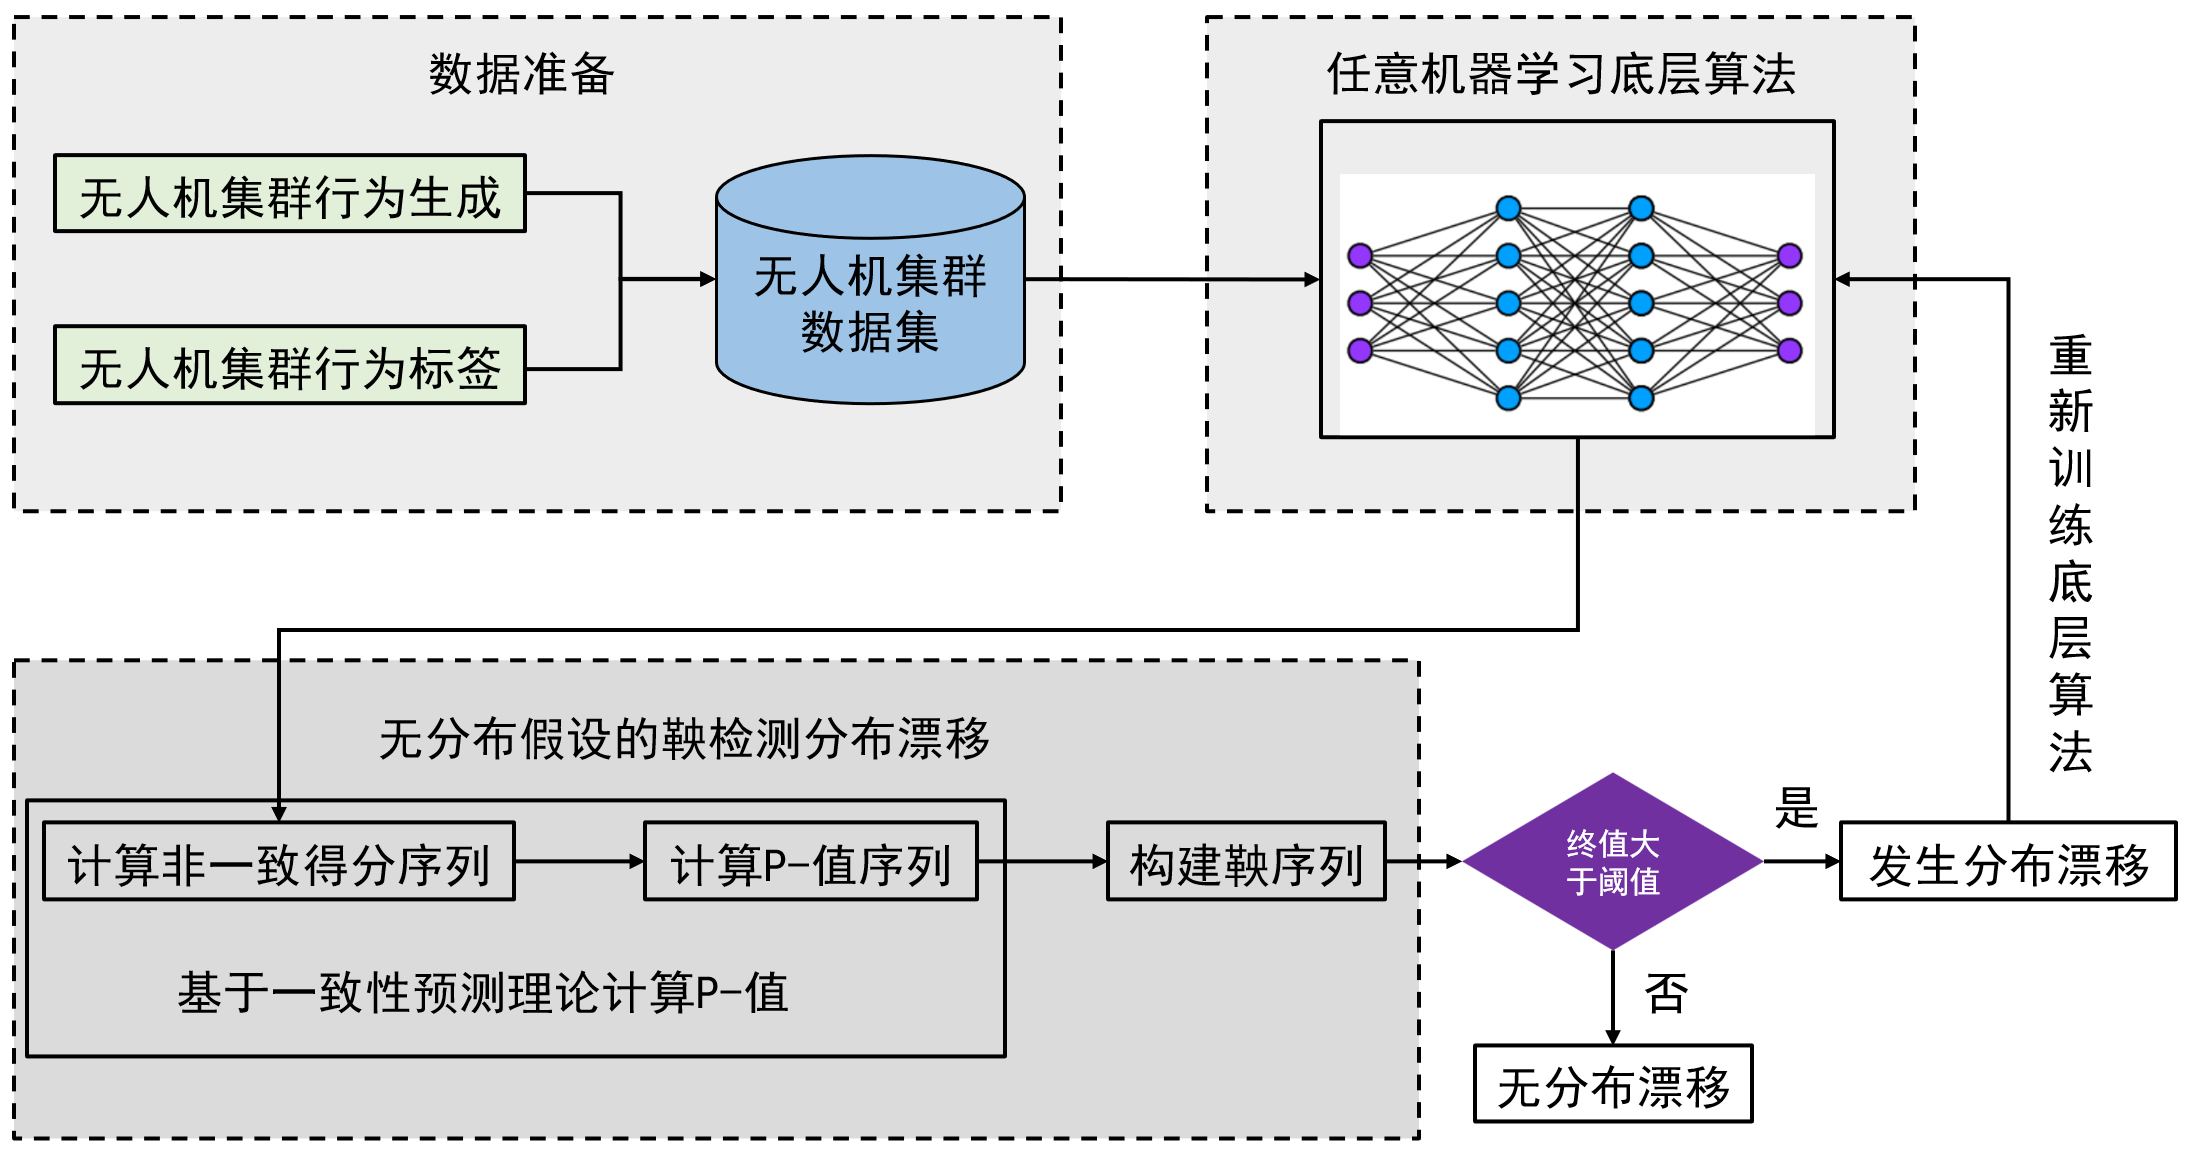
\includegraphics[width=1\linewidth]{Img/martingale.png}}
\caption{无分布假设鞅序列分布漂移检测方案框架图}
\label{fig:martingale}
\end{figure*}

本文针对真实无人机集群行为数据展开分布漂移检测。因此在数据准确阶段直接采用第\ref{chap:Swarm-MCP}章中的公开无人机集群行为数据集作为研究对象, 并且在构建底层机器学习算法时严格按照数据本身的时间顺序将无人机集群数据划分为训练集和测试集。使用训练集得到学习模型后, 便可以利用此学习模型得到测试数据集的预测结果, 然后根据机器学习预测输出结果构建分布漂移检测方法。

本文提出的分布漂移检测方法是建立在机器学习模型之上的, 因此, 可以选取任意的机器学习模型作为底层算法。选择三种具有代表性的现代机器学习算法, 分别是全连接神经网络算法,Boosting算法和支持向量机算法。根据训练数据得到机器学习算法的参数设定后, 底层机器学习算法被视为超越算子, 因此测试数据经过超越算子后被压缩为单个值, 本文提出的分布漂移检测算法就是基于此压缩值而展开分析的。

在第\ref{chap:edbed}章和第\ref{chap:Swarm-MCP}章中已经阐明, 机器学习算法的输出结果仅仅表征样本之间的相似度\citep{vapniktalk2022}, 因此需要利用一致性预测理论计算其对应的非一致性得分。进而根据通过一致性预测得到经验数据对应的p-值序列\citep{2006Hedging}, 然后基于计算得到的p-值序列构建权力鞅(power martingales)序列\citep{Ville1939}。权力鞅序列的构建无需任何分布假设, 因此称之为无分布假设的鞅序列检测分布漂移方法(Distributions-free Martingales Test Distributions-shift)。 

基于已有的鞅理论\citep{glenn-vovk2001,glenn-vovk2019}, 所构建的权力鞅序列能够实现分布漂移检测的任务。根据鞅理论的研究成果, 本文提出一旦权力鞅序列的取值超过某个提前给定的阈值(此阈值根据鞅理论, 取值一般在20-100之间。本文将此阈值设定在最宽松情形下, 即阈值设定为100), 就认为此时的底层机器学习算法对后续测试数据无法提供高效的预测, 认定此时数据发生分布漂移。

然而, 尽最大努力调研文献之后发现很少有研究关注到当利用机器学习算法处理真实无人机集群行为预测时, 考虑对无人机集群行为数据本身分布漂移的检测研究。即很少有研究关注到如何对机器学习模型的条件假设给出检测的问题。 这就是说, 利用机器学习算法确实能够实现真实数据的分类, 这些优良的分类结果大都建立在默认将数据随机采样得到训练集和测试集, 然后利用训练集得到预测模型, 进而在测试数据集上展开预测分析。

但本章考虑的问题是: 如果不进行随机采样, 严格按照实际工程数据的真实顺序划分训练集和数据集。在不随机采样数据的要求下, 利用训练集训练模型, 并在测试集上检验模型的预测能力。在这种情形下就需要检测所得机器学习模型是否会继续保持优质的预测能力。如果随机采样数据不会对机器学习算法预测能力产生较大影响, 那么真实数据没有发生分布漂移, 因此研究者可以继续使用先前训练模型为后续测试样本提供预测。如果对比随机采样数据前后机器学习模型预测能力有较大差距, 这说明数据本身的时间顺序是值得被关注的研究对象, 因此分布漂移检测就能够为机器学习算法预测能力提供一种预警。  

就文献调研所知, 第一个针对实际数据展开分布漂移的研究是由\citet{Vovk2003}在考虑USPS手写数字问题中提出的。 \citet{Vovk2003}考虑针对美国国家邮政局(U.S. Postal Service, USPS)提供的手写数字识别展开研究。 此数据集一共包含9298个16$\times$16像素灰度的手写数字, 此数据集保留美国国家邮政局收集数据时的时间顺序\citep{vovk-pvalue2019}。 Vovk将自己提出的鞅方法应用到原初USPS数据集上发现, 机器学习对于随机化数据和按照真实数据顺序这两种情形的学习推广能力有巨大的差别。

根据Bruno de Finetti现代概率论批判理论可知\citep{Finetti1975}, 分布漂移检测问题更一般的理论陈述是“随机变量可交换性检测”问题\citep{Finetti1975}。\citet{Vovk2003}提出使用鞅序列方法检测随机变量的可交换性并且指出对于实际工程问题, 数据的可交换性假设通常是被拒绝的, 即对于实际工程应用中的真实数据, 是不满足可交换性假设的。换言之, Bruno de Finetti现代概率论批判理论指出, 在自然科学研究中应该严格按照数据本身的顺序展开模型构建, 而不应该将数据随机化操作后再构建学习模型。 

受此启发, 在研究无人机集群行为分类这一实际应用工程问题时也探讨随机化无人机集群行为数据带来的影响。 经过文献调研后发现, 在无人机集群行为分类研究中, 鲜有文献对这一问题展开研究, 然而在其他应用研究领域, 已经有学者应用鞅理论处理实际工程应用。 例如, \citet{Ho2005} 将权力鞅序列理论应用于时变流的变点检测问题上, 并且指出对于任意的机器学习算法, 权力鞅序列给出的分布漂移检测结果能够灵敏检测数据分布的变化, 为时变流工程应用提供切实可信的数据支撑。\citet{Ho2012} 也在变点检测理论中提出可交换性检测的概念, 他的研究结果表明在变点检测问题中, 基于鞅序列的检测方法能够精确给出研制问题的解, 并且可以针对超高维数据展开精确有效的变点检测。 \citet{Ho2019}将鞅序列检测理论成功地应用于飞行器行为的异常检测项目。这些研究表明对于实际工程应用研究, 鞅方法能够为研制问题提供端到端的解决方案。因此, 提出为无人机集群实际工程数据也开展分布漂移检测。

\section{基于一致性预测的鞅序列构建}

本节首先对基于鞅方法的分布漂移检测理论进行介绍。分布漂移检测是可交换性检测的一个特例, 因此, 在Bruno de Finetti现代概率论批判意义下很容易获得分布漂移检测方案。 考虑给定随机变量序列$(Z_1,Z_2,\ldots)$, 其对应的具体输出元素成为样例序列$(z_1, z_2,\ldots)$, 其中每个样例都由两部分组成, 即对象$x_i$和对应的标签$y_i$。 给定原假设: 样例序列$(z_1, z_2, \ldots)$都是根据某个固定的且未知的概率分布函数$P(x)$生成, 即
\begin{center}
\textsf{原假设 $H_0$}: 样例序列没有发生分布漂移。
\end{center}

提出的分布漂移检测方法分为三步完成。 首先根据训练数据训练底层机器学习算法, 按照实际数据本身的时间顺序将数据划分为训练集和测试集。得到底层机器学习算法后, 计算测试数据的预测输出得分。根据第\ref{chap:edbed}章和第\ref{chap:Swarm-MCP}章的阐述可知, 机器学习算法的输出结果仅仅是样本相似程度的度量, 并且只有经过一致性预测算法校正后才能够有效控制错误误差。因此, 第二步需要根据机器学习算法预测输出计算非一致性得分, 进而得到每个样本对应的p-值得分函数。第三步, 根据p-值得分函数结合鞅理论可以构建权力鞅序列。根据鞅理论的研究成果, 权力鞅序列的最终取值不可能过大, 如果权力鞅序列的最终取值超过给定的阈值, 就可以依概率拒绝零假设, 即判定样例序列可能发生分布漂移。

\subsection{基于一致性预测算法计算p-值}
设样例$(z_1,z_2,\ldots)$按照原始顺序依次收集, 根据第\ref{chap:Swarm-MCP}章介绍的一致性预测理论知识, 首先借助底层机器学习算法得到每个样本的预测输出。由于机器学习算法的预测输出仅仅是相似度度量, 需要将每个相似度度量函数按照一致性预测理论计算非一致性得分。一致性预测扮演的角色是将底层机器学习输出的未校正相似度度量函数校正为有效相似程度度量函数。 非一致性得分函数定义为
\begin{align}
\label{alpha-4.1}
\alpha_{i} = A_{n}(\{z_1,\ldots,z_{i-1},z_{i+1},\ldots,z_{n}\}, z_{i}),
\end{align}

根据\citet{vapnik1995,vapnik1998}提出的超越推理理论, 机器学习算法将经验事实以超越推理范式映射至函数的值。因此, 可以选择任意的机器学习算法作为底层超越算子。采用三种经典学习模型作为底层机器学习算法(分别是SVMs, Boosting算法和神经网络算法)计算非一致性得分。

具体而言, 非一致性得分函数的定义可以有众多不同的方法, 中选择逆概率作为非一致性测度函数\citep{Johansson2017}, 即
\begin{align}
\label{alpha-4.2}
\alpha_{i} = - \hat{p}_{i}.
\end{align}
其中, $\hat{p}_{i}$是底层机器学习算法输出的“概率值”。

根据计算得到的非一致得分函数可以快速构建p-值函数序列\citep{vovk2005algorithmic}。通常而言, 可以通过标准化非一致得分来计算p-值函数序列, 即对于样本$z_n$所对应的p-值序列, 按照下列表达式计算可以得到有效的p-值序列
\begin{align}
\label{alpha-4.3}
p_n = \frac{\#\{i: \alpha_i > \alpha_n\} + \tau_n \# \{i: \alpha_i = \alpha_n\}}{n}.
\end{align}
其中, 这里$\tau_n$是随机化因子, 其服从于$[0, 1]$上的均匀分布, 符号 \# 表示集合大小的测度。 显而易见对于任意的底层算法, 根据上述一致性预测方法计算得到的p-值函数是精确有效的, 即根据这种方法计算得到的p-值序列严格服从$[0,1]$上的均匀分布。关于这一陈述的证明参见定理\ref{theorem}, \citet{vovk2005algorithmic}给出关于此定理的证明。

\begin{theorem}
\label{theorem}
如果样例$(z_1,z_2,\ldots)$满足可交换性假设, 那么p-值序列都是独立的并且服从$[0,1]$上的均匀分布。
\end{theorem}
p-值序列精确有效的性质是非常重要的, 因为从统计学理论的要求来看, 借助一致性预测方法生成的精确有效p-值序列为后续展开有效的统计推断提供严格的理论保证。

\subsection{基于p-值构建鞅序列}
\label{sec:aglorithm}
本节详细介绍基于一致性预测校正后有效p-值序列构建鞅方法检测分布漂移。首先, 基于鞅理论设定博弈函数(betting function), 此函数满足鞅理论要求。利用博弈函数的映射关系可以得到每个p-值序列对应的博弈函数取值。权力鞅序列定义为博弈函数取值的乘积。由于给定的博弈函数满足$[0, 1]$上的积分为1, 所以构建得到的权力鞅序列可以视为分布漂移的量化标识。根据鞅理论要求, 如果没有发生分布漂移, 权力鞅序列的取值会一直衰减。换言之, 如果没有发生分布漂移, 权力鞅不会取得较大的值。因此, 仅仅根据权力鞅最终的取值大小即可做出是否拒绝零假设的判断。

具体而言, 对于每个样例$i \in \{1,2,\ldots\}$, 设下列函数
\begin{align}
f_i : [0,1]^{i} \rightarrow [0, \infty)
\end{align}
是给定的博弈函数, 此函数将服从$[0,1]$上的均匀分布随机变量映射至非负取值变量, 并且定义函数满足下列表达式,
\begin{align}
\label{betting}
\forall i: f(p_i) = \varepsilon p_{i}^{\varepsilon -1}.
\end{align}
其中, 这里$\varepsilon \in [0,1]$。对于博弈函数$f(x)$, 要求满足下列表达式
\begin{align}
\int_{0}^{1}f(x)dx=1.
\end{align}
根据博弈函数, 满足下列表达式的随机序列定义为权力鞅序列, 
\begin{align}
M_{n}^{(\varepsilon)} := \prod_{i=1}^{n}(\varepsilon p_{i}^{\varepsilon - 1}),
\end{align}
其中, 这里的 $p_1, p_2, \ldots, p_n$是借助一致性预测方法计算得到的p-值序列, 此序列是以初始值为1的非负的、被随机化后的鞅序列。 这一类鞅序列称为随机化的权力鞅序列(randomised power martingales), 简称权力鞅序列。

根据鞅理论\citep{Ville1939,Doob1984}, 满足零假设的鞅序列满足下列表达式
\begin{align}
\label{alpha-4.7}
M_{n} \geq E(M_{n+1} | \mathcal{F}_{n}),
\end{align}
其中, 这里$\mathcal{F}_{n}$是由序列$z_{1}, \ldots, z_{n}$生成的$\sigma$-代数。如果$M_{0}=1$并且$\inf_{n}M_{n} \geq 0$, 那么随机过程$M_{0}, M_{1}, \ldots$被定义为资本过程\citep{Vovk1993,vovk2001,vovk2021,Bienvenu2022,Laurent2009,Bienvenu2009OnTH}。“资本过程”这一术语形象地阐述分布漂移检测理论的思想, 即按照鞅理论此资本过程表示赌徒从单位资产出发, 每次都押注: “按照公平的自然选择, 所得的结果$M_{n}$并不会使自己破产”。按照鞅理论来理解学习过程, 即每次都押注: “按照机器给出的结果预测测试样本, 那么测试样本对应的预测结果在总体上不会大面积出错”。所以测试样本对应的权力鞅序列$M_{n}$就不可能取得一个较大的值。这就表明, 依靠训练数据得到的机器学习模型仍然能够为测试数据提供预测, 即测试数据的分布没有发生漂移。

根据鞅理论\citep{Ville1939,Doob1984}, 满足零假设的鞅序列满足下列表达式
\begin{align}
\label{martingale-C}
P\{\forall n: M_{n} \geq C\} \leq \frac{1}{C},
\end{align}
其中, $C$是任意取值为正的常数。 此条件表明, 当数据没有发生分布漂移时, 鞅序列不会取得较大的值。因此, 在分布漂移检测方法中, 如果数据对应的鞅序列取得较大值, 那么就可以依概率拒绝零假设, 认为发生分布漂移。算法 \ref{alg:on-line-testing} 给出整个无分布假设鞅实现分布漂移的检测算法(Distributions-free Martingale Test Distributions-shift, DFMTDS)。

\begin{algorithm}[!htbp]
    \small
    \caption{无分布假设的鞅检测分布漂移算法(DFMTDS)}
    \label{alg:on-line-testing}
    \hspace*{\algorithmicindent} \textbf{输入:} {$z_{i}, i=1,\ldots,n$, 底层算法$T$, $\epsilon$.}\\
    \hspace*{\algorithmicindent} \textbf{输出:} {鞅序列的终值$M_{n}$.}
    \begin{algorithmic}[1]
        \Procedure{DFMTDS}{}
        \State 利用训练数据集训练学习模型$T$,
        \For{$i=1$ {\bfseries to} $n$}
        \State 使用表达式(\ref{alpha-4.2})计算 $\alpha_i$,
        \State 使用表达式(\ref{alpha-4.3})计算 $p_i$,
        \State 使用表达式(\ref{alpha-4.7})计算 $M_{i}$,
        \EndFor
        \While{$M_{n} \leq \epsilon$}
        \State 根据表达式(\ref{martingale-C})返回 $M_{n}$.
        \EndWhile
        \EndProcedure
    \end{algorithmic}
\end{algorithm}

\section{基于鞅序列的无人机集群数据分布漂移检测}
\label{empiricaldtudies}
本节详细介绍针对无人机集群行为数据的分布漂移检测。对比随机采样无人机集群行为数据和按照无人机集群行为数据本身时间顺序这两种模式下的分布漂移检测。首先介绍本章测试算例所用到的数据集并且对比随机化采样数据前后训练所得机器学习模型的预测能力; 然后按照提出的鞅方法计算在保留无人机集群行为数据本身时间顺序建模情形下, 计算鞅序列的取值; 最后按照提出的鞅方法计算随机化处理无人机集群行为数据的鞅序列。

将无人机集群行为分布漂移检测算法应用于三种公开的真实无人机集群行为数据进行检测。无人机集群行为数据的分布漂移可以通过对比随机化数据前后机器学习算法的鞅序列取值来检测。如果无人机集群行为数据没有发生分布漂移, 那么随机化数据并不会对机器学习的预测效果产生影响,对应的鞅序列取值不会大于给定的阈值。

分别针对三种无人机集群行为真实数据(即Align行为数据集, Flock行为数据集和Group行为数据集)开展分布漂移检测问题。 提供三种机器学习算法作为底层算法并且通过对比三种机器学习算法对应的权力鞅序列的取值实现分布漂移检测。

无人机集群行为数据集已经在第\ref{chap:Swarm-MCP}章已经介绍过, 本章将数据集合划分为6004个训练样本, 剩余的18011个样本作为测试样本。 需要特别注意的是, 本章默认按照保留数据本身的时间顺序划分训练集和测试集。 如第\ref{chap:Swarm-MCP}章所述, 每个样本的属性描述在第\ref{chap:Swarm-MCP}章的表\ref{tab:datainfo}中列出, 本章所用到的数据划分方式在表\ref{tab:train_test1}中给出, 本章仍然仅选择位置坐标作为输入变量。

% Please add the following required packages to your document preamble:
% \usepackage{booktabs}
\begin{table}[]
\centering
\caption{无人机集群三种典型行为训练集和测试集信息汇总表}
\label{tab:train_test1}
\begin{tabular}{@{}llll@{}}
\toprule
数据集 & 维数  & 训练样本数 & 测试样本数  \\ \midrule
Align    & 2400 & 6004     & 18011 \\
Flock    & 2400 & 6004     & 18011 \\
Group    & 2400 & 6004     & 18011 \\ \bottomrule
\end{tabular}
\end{table}

\subsection{随机处理数据前后对比研究}

在开展分布漂移检测之前, 首先对比按照数据本身时间顺序建模和随机化数据建模情形下, 机器学习算法的预测能力。按照表\ref{tab:train_test1}要求下划分训练数据和测试数据。使用前6004个样本训练三种机器学习算法, 然后使用机器学习算法预测后18011个测试样例。表\ref{tab:online}展示有序学习模式下错误分类的数目。从表\ref{tab:online}可以看到, 对于Align行为数据集, 全连接神经网络算法(MLP)预测错误的数目最小; 对于Flock行为数据集, Boosting算法预测错误的数目最小; 对于Group行为数据集, Boosting算法预测错误的数目最小。纵观表\ref{tab:online}中预测错误数目, 发现在保持数据本身时间顺序后, 这三种机器学习算法都并没有表现出极其优越的预测效果。

% Please add the following required packages to your document preamble:
% \usepackage{booktabs}
% \usepackage{graphicx}
\begin{table}[]
\centering
\caption{无人机集群有序学习的预测错误数目汇总表}
\label{tab:online}
\begin{tabular}{@{}llll@{}}
\toprule
数据集   & SVMs预测错误数目 & MLP预测错误数目 & Boosting预测错误数目 \\ \midrule
Align & 1492       & 848       & 1763           \\
Flock & 2928       & 2125      & 2055           \\
Group & 1385       & 1031      & 452            \\ \bottomrule
\end{tabular}%
\end{table}


然而, 如果仅仅在构建模型之前将真实无人机集群行为数据随机处理, 然后再同样按照表\ref{tab:train_test1}中要求划分训练集和测试集。仍然利用训练集得到三种机器学习算法, 两种情形所用的三种底层机器学习算法均采用默认参数。在这种情形下, 与上述唯一不同之处就在于在开展划分训练集和测试集之前, 对数据先行进行随机化处理。 表\ref{tab:offline}展示随机化后三种机器学习算法在三种随机化处理后的无人机集群行为数据集上的预测效果。很明显, 当随机化处理数据后, 三种机器学习算法对于三种无人机集群行为数据都给出相当优越的预测效果。

% Please add the following required packages to your document preamble:
% \usepackage{booktabs}
% \usepackage{graphicx}
\begin{table}[]
\centering
\caption{无人机集群随机化后学习的预测错误数目汇总表}
\label{tab:offline}
\begin{tabular}{@{}llll@{}}
\toprule
数据集   & SVMs预测错误数目 & MLP预测错误数目 & Boosting预测错误数目 \\ \midrule
Align & 1          & 0         & 1              \\
Flock & 0          & 2         & 1              \\
Group & 1          & 2         & 1              \\ \bottomrule
\end{tabular}%
\end{table}


具体而言, 对于Align数据集, 随机化处理前SVMs算法预测错误数目是1492, 随机化后预测错误数目是1; 随机化处理前全连接神经网络算法预测错误数目是848, 随机化后预测错误数目是0; 随机化处理前Boosting算法预测错误数目是1763, 随机化后预测错误数目是1。对于Flock数据集, 随机化处理前SVMs算法预测错误数目是2918, 随机化后预测错误数目是0; 随机化处理前全连接神经网络算法预测错误数目是2125, 随机化后预测错误数目是2; 随机化处理前Boosting算法预测错误数目是2055, 随机化后预测错误数目是1。对于Group数据集, 随机化处理前SVMs算法预测错误数目是1385, 随机化后预测错误数目是1; 随机化处理前全连接神经网络算法预测错误数目是1031, 随机化后预测错误数目是2; 随机化处理前Boosting算法预测错误数目是452, 随机化后预测错误数目是1。

显而易见, 对于实际工程中的无人机集群数据集, 随机化处理数据前后机器学习算法的预测能力具有数量级层面的差距。这一方面说明对于实际数据, 可以通过采用随机化处理数据来实现更高精度的预测, 但是同时也说明, 如果需要按照实际工程数据自身时间顺序建模(例如在实际工程中遇到有序学习任务时, 无法提供随机化真实数据的条件), 那么对于实际数据需要额外关注机器学习算法预测能力的边界。因为随着实际数据本身时间顺序的积累, 数据本身的分布是研究者不得不考虑的重要信息。正因为注意到随机化前后机器学习算法的预测能力所表现的这种巨大差距, 提出对真实无人机集群数据展开分布漂移检测。

\subsection{无人机集群行为数据分布漂移检测}
本节研究利用无分布假设的鞅方法检测无人机集群数据的分布漂移, 以验证对于实际工程中真实无人机集群数据, 所提方法能够高效地指示出分布发生变化的位点。这种方法能够为研究者提供一种提示信息, 即当鞅序列的终值大于给定阈值时, 表明利用先前训练数据得到的机器学习算法已经无法为分布发生变化的测试数据继续提供高效准确的预测, 应该在此时重新训练模型, 以获得更高效的预测性能。根据鞅序列理论, 表达式(\ref{martingale-C})中常数$C$的取值一般选取为$[20, 100]$, 选择最宽松的情形, 即$C=100$。也就是说, 在最宽松的要求下检测真实无人机集群数据是否会有分布漂移的发生。

首先, 对于Align数据集, 图\ref{fig:align-mar}展示三种机器学习算法计算得到的鞅序列。图\ref{fig:align-mar}展示学习样本按照原始顺序进入模型后权力鞅序列的增长情形。 例如, 当采用全连接神经网络作为底层算法时(图示中的“MLP”表示全连接神经网络算法), 权力鞅序列最终的取值大约是$114$, 权力鞅的最终值大于给定的阈值100。对于SVMs算法和Boosting 算法, 其最终的取值分别大约是$246$和$267$, 这两个取值是远远大于给定的阈值100。 这说明对于无人机集群行为数据集, 如果按照数据本身时间顺序建模, 那么在训练集上得到的机器学习算法其泛化推广能力是有边界的。换言之, 大概第14000个样本左右(此时权力鞅的取值达到阈值100左右), 在训练集上得到的机器学习算法无法为分布已然发生变化的测试数据继续提供准确高效的预测。如果研究者想要获得准确高效的预测, 就应该在分布发生变化的第14000个样本左右重新训练机器学习模型。权力鞅的检测结果也证实表\ref{tab:online}中Align数据集的预测表现, 即在保留数据本身顺序情形下构建的机器学习算法并没有提供极其优越的预测效果。

图\ref{fig:align-mar}也表明对于不同的机器学习算法, 其对分布漂移展示出不同程度的鲁棒性。对于Align数据集, 图\ref{fig:align-mar}显示SVMs算法和Boosting算法大致在第14000个测试样本左右达到阈值, 而神经网络算法的学习泛化能力强于SVMs算法和Boosting算法, 大概在第17000个样本达到此阈值。 这意味着对于保持原本顺序Align行为的无人机集群数据集, SVMs算法和Boosting算法比全连接神经网络算法对于分布漂移检测更敏感。 换言之, 从另一方面也说明神经网络算法相较于其他两个算法具有更强的泛化推广能力。

图\ref{fig:radom-align-mar}展示三种机器学习算法在随机化处理后的Align数据集上计算得到的鞅序列。图\ref{fig:radom-align-mar}展示此情形下权力鞅序列的增长情形。图中结果表明随机处理Align数据集后三种机器学习算法的权力鞅序列都没有大于阈值100, 因此可以判定在这种情形下三种机器学习算法都可以提供相当优越的预测结果。权力鞅的检测结果也证实表\ref{tab:offline}中Align数据集的预测表现, 即随机化后的机器学习算法都提供优越的预测效果。

图\ref{fig:radom-align-mar}也表明即便利用随机采样的训练集构建机器学习模型可以得到相当满意的预测效果, 但是鞅序列仍然是保持了向上增长的趋势, 并且如果持续增加测试样本, 此序列也会缓慢超过给定阈值。这说明即便随机采样后数据满足独立同分布假设, 但是数据本身的分布漂移仍然是存在的。

\begin{figure*}[htbp] % [tb]
\centerline{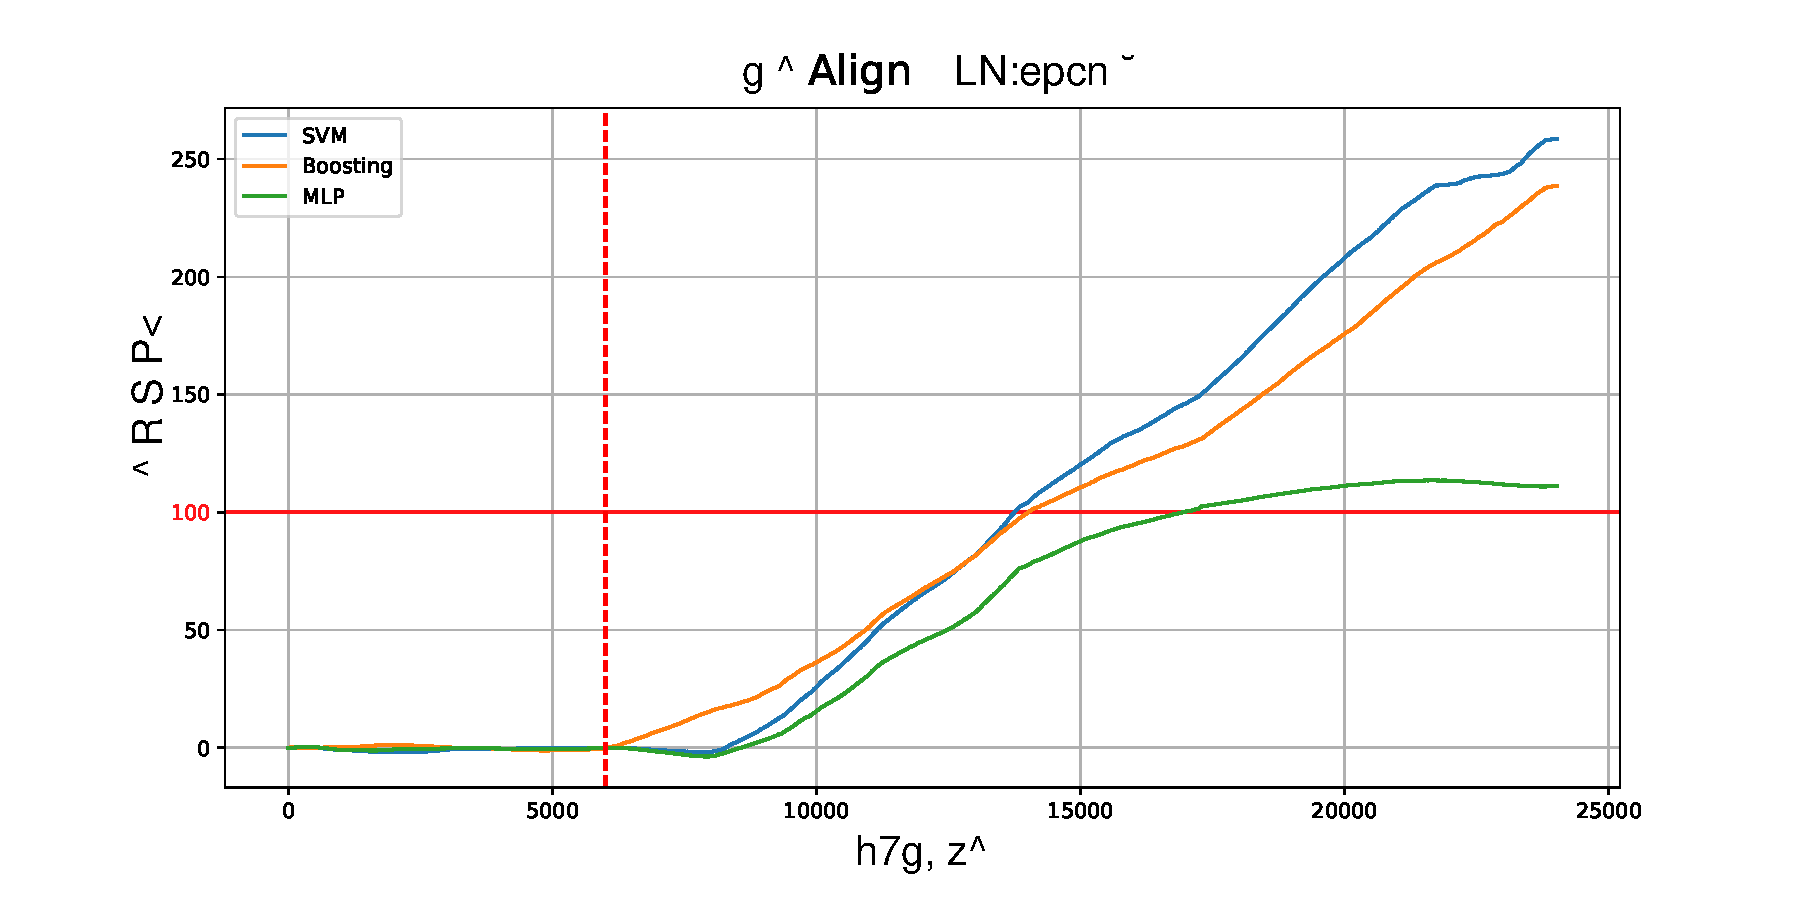
\includegraphics[width=1\linewidth]{Img/chapter9/Align data set-icml}}
\caption{{Align}行为数据集有序学习的鞅序列}
\label{fig:align-mar}
\end{figure*}
\begin{figure*}[htbp] % [tb]
\centerline{
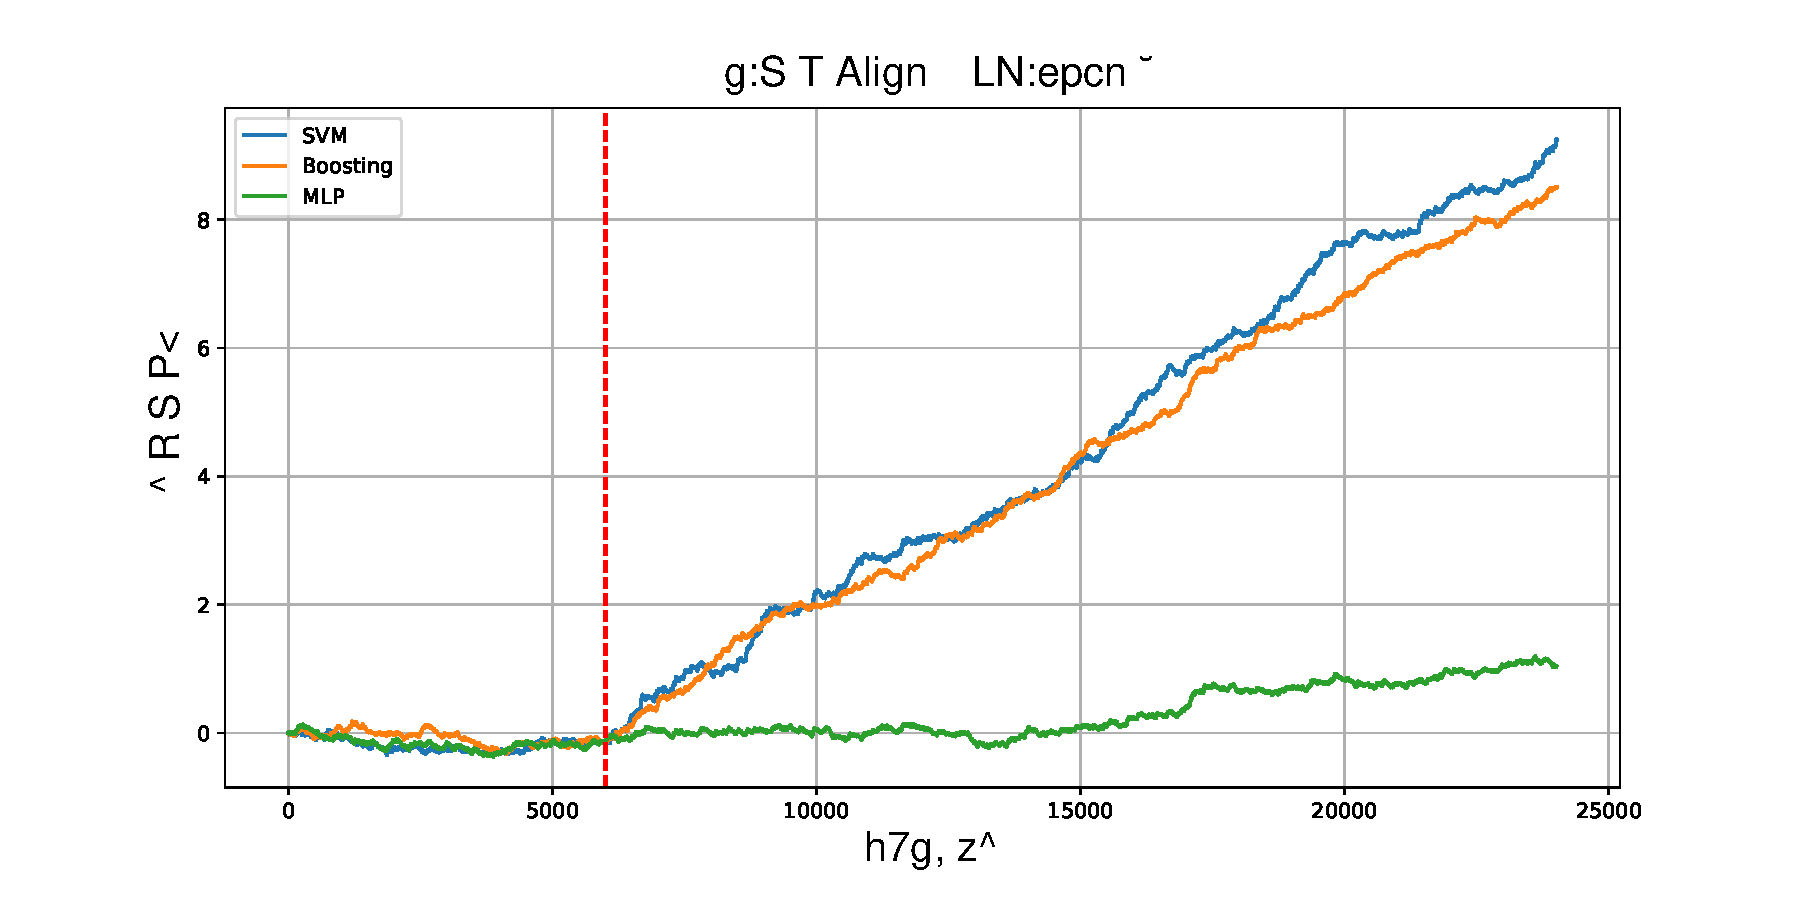
\includegraphics[width=1\linewidth]{Img/chapter9/Randomly shuffling Align data sett-icml}}
\caption{随机化{Align}行为数据集有序学习的鞅序列}
\label{fig:radom-align-mar}
\end{figure*}


其次, 对于Flock数据集, 图\ref{fig:flock-mar}展示三种机器学习算法计算得到的鞅序列。图\ref{fig:flock-mar}展示学习样本按照原始顺序进入模型后权力鞅序列的增长情形。 例如, 当采用全连接神经网络作为底层算法时, 权力鞅序列最终的取值大约是$210$, 权力鞅的最终值远远大于给定的阈值100。对于SVMs算法和Boosting 算法, 其最终的取值分别大约是$390$和$320$, 这两个取值也是远远大于给定的阈值100。 这说明对于Flock行为的无人机集群行为数据集, 如果按照数据本身时间顺序建模, 那么在训练集上得到的机器学习算法一定不能一直被当作“万能逼近”算子采用, 而应该在鞅序列大于阈值100处停下来。换言之, 对于Flock数据集而言, 如果采取保守策略, 对于SVMs算法和Boosting算法应该在大概第12000个测试样本左右(此时权力鞅的取值第一次达到阈值100左右)停止使用先前训练的机器学习算法; 对于神经网络算法大概应该在第14000个测试样本左右停止使用先前训练得到的算法。权力鞅的检测结果也证实表\ref{tab:online}中Flock数据集的预测表现, 即在保留数据本身顺序情形下构建的机器学习算法并没有提供极其优越的预测效果。

同样, 图\ref{fig:flock-mar}也表明对于不同的机器学习算法对Flock数据集的分布漂移展示出不同程度的鲁棒性。根据达到阈值100的样本量大小可知神经网络算法对于Flock数据集表现出更稳健的预测效果。但是由于鞅序列表达式(\ref{martingale-C})给出的结果是基于“依概率(in probability)”的结论, 所以神经网络在总体上的预测效果并没有比Boosting算法优越。然而对于分布漂移检测问题, 则可以肯定鞅序列方法提供高效的检测能力。

图\ref{fig:radom-flock-mar}展示三种机器学习算法在随机化处理后的Flock数据集上计算得到的鞅序列。图\ref{fig:radom-flock-mar}展示此情形下权力鞅序列的增长情形。图中结果表明随机处理Flock数据集后三种机器学习算法的权力鞅序列都没有大于阈值100, 因此可以判定在这种情形下三种机器学习算法都可以提供相当优越的预测结果。权力鞅的检测结果也证实表\ref{tab:offline}中Flock数据集的预测表现, 即随机化后的机器学习算法都提供优越的预测效果。

图\ref{fig:radom-flock-mar}更明显地表明即便利用随机采样的训练集构建机器学习模型可以得到相当满意的预测效果, 但是鞅序列仍然是保持了向上增长的趋势, 并且如果持续增加测试样本, 此序列也会缓慢超过给定阈值 (如果将阈值设定为更为严格的$C=20$, 那么SVMs算法下就已经指示出随机采样后的Flock数据也存在分布漂移)。这说明即便随机采样后数据满足独立同分布假设, 但是数据本身的分布漂移仍然是存在的。

\begin{figure*}[htbp] % [tb]
\centerline{
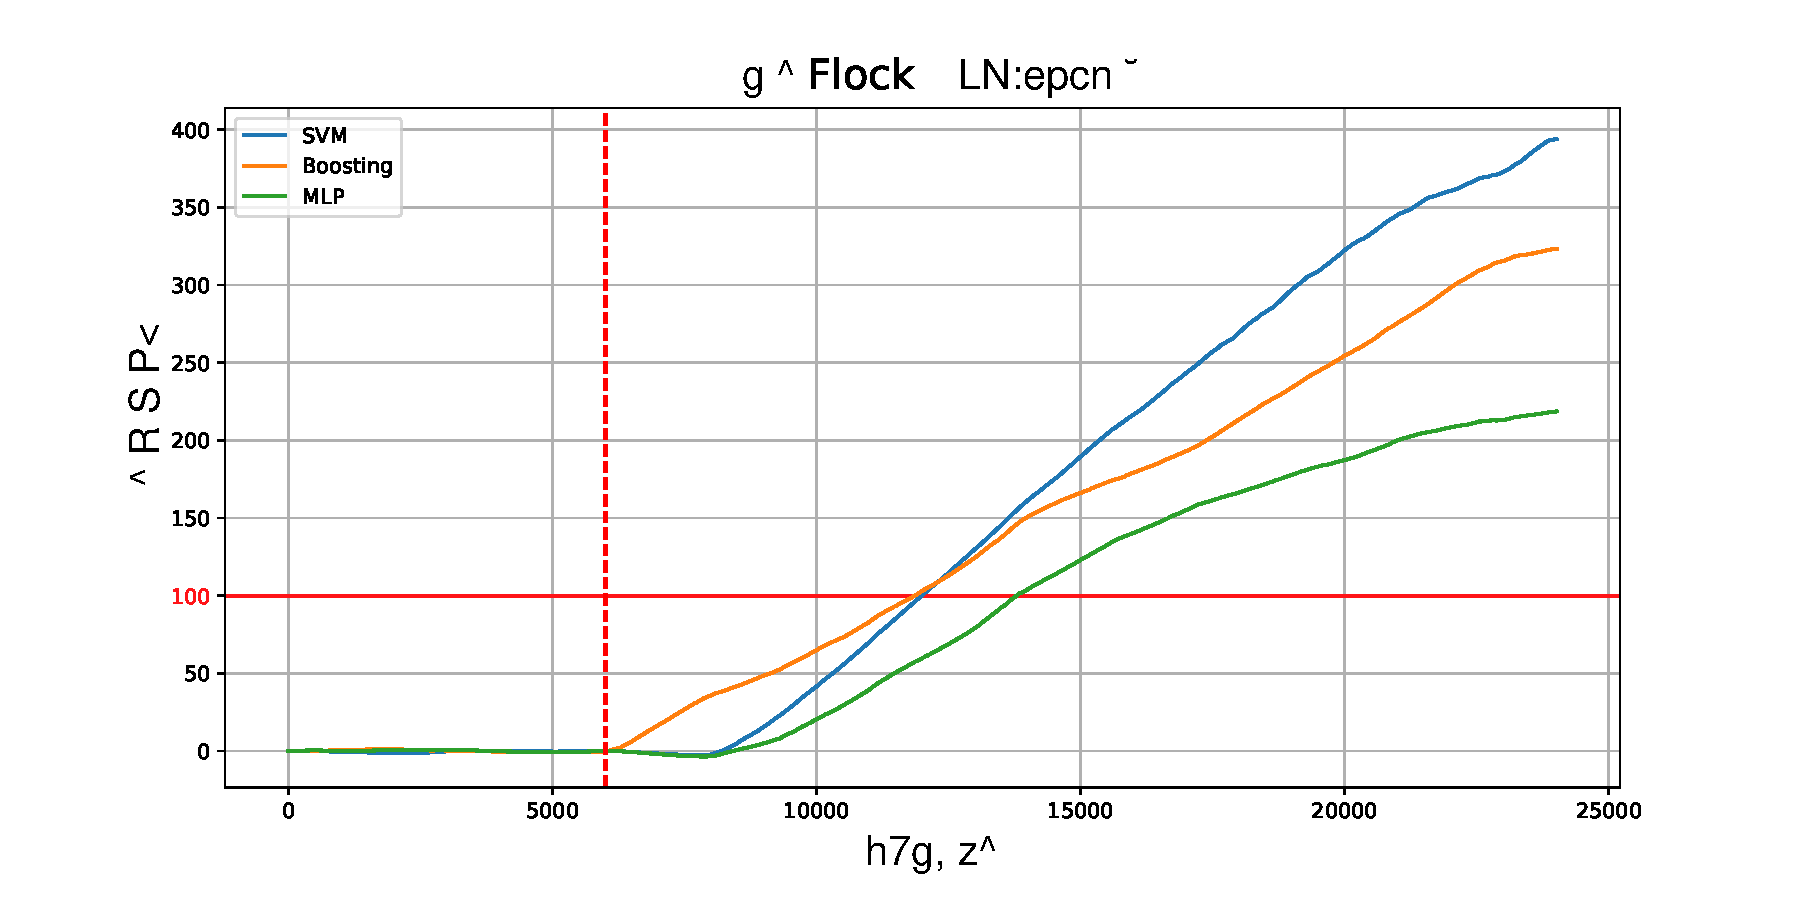
\includegraphics[width=1\linewidth]{Img/chapter9/Flock data set-icml}}
\caption{{Flock}行为数据集有序学习的鞅序列}
\label{fig:flock-mar}
\end{figure*}
\begin{figure*}[htbp] % [tb]
\centerline{
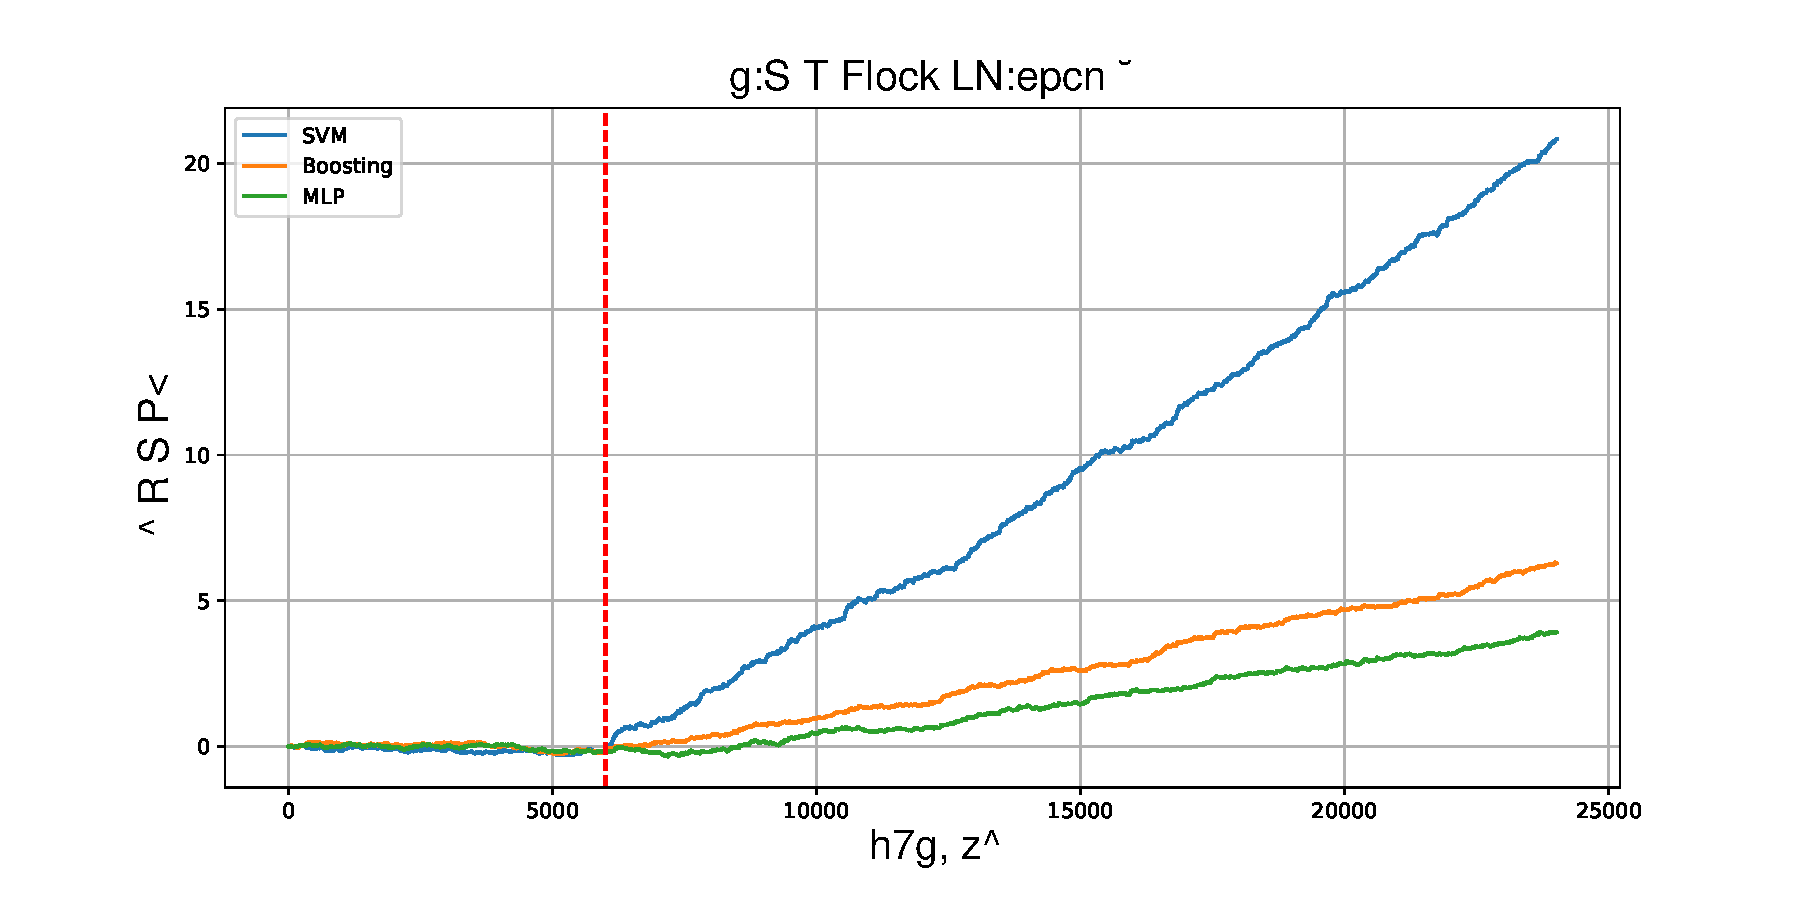
\includegraphics[width=1\linewidth]{Img/chapter9/Randomly shuffling Flock data sett-icml}}
\caption{随机化{Flock}行为数据集有序学习的鞅序列}
\label{fig:radom-flock-mar}
\end{figure*}


最后, 对于Group数据集, 图\ref{fig:group-mar}展示三种机器学习算法计算得到的鞅序列。当底层算法是Boosting时最先达到阈值100, 此时大约在第12000个样本达到阈值; 其次是SVMs算法, 其大约在第13000个样本时达到阈值100; 而当底层算法是神经网络算法时, 一直要持续到第15000个样本以后, 才达到阈值100。 这就是说, 对于Group数据集, 当底层算法是Boosting时, 大约在第12000个样本左右就可以拒绝零假设; 当底层算法是SVMs时, 大约在第13000个样本左右就可以拒绝零假设; 而底层算法是神经网络时, 一直到大约在第15000以后的样本才可以拒绝零假设。权力鞅的检测结果也证实表\ref{tab:online}中Group数据集的预测表现, 即在保留数据本身顺序情形下构建的机器学习算法并没有提供极其优越的预测效果。

与先前两种无人机集群行为数据相似, 图\ref{fig:radom-group-mar}展示三种机器学习算法在随机化处理后的Group数据集上计算得到的鞅序列。图\ref{fig:radom-group-mar}展示此情形下权力鞅序列的增长情形。图中结果表明随机处理Group数据集后三种机器学习算法的权力鞅序列都没有大于阈值100, 因此可以判定在这种情形下三种机器学习算法都可以提供相当优越的预测结果。权力鞅的检测结果也证实表\ref{tab:offline}中Group数据集的预测表现, 即随机化后的机器学习算法都提供优越的预测效果。

图\ref{fig:radom-group-mar}也表明即便利用随机采样Group数据集得到的训练集构建机器学习模型可以得到相当满意的预测效果, 但是鞅序列仍然是保持了向上增长的趋势, 并且如果持续增加测试样本, 此序列也会缓慢超过给定阈值(在随机化后的Group数据集中, SVMs最终取值达到17.5)。这说明即便随机采样后数据满足独立同分布假设, 但是数据本身的分布漂移仍然是存在的。

\begin{figure*}[htbp] % [tb]
\centerline{
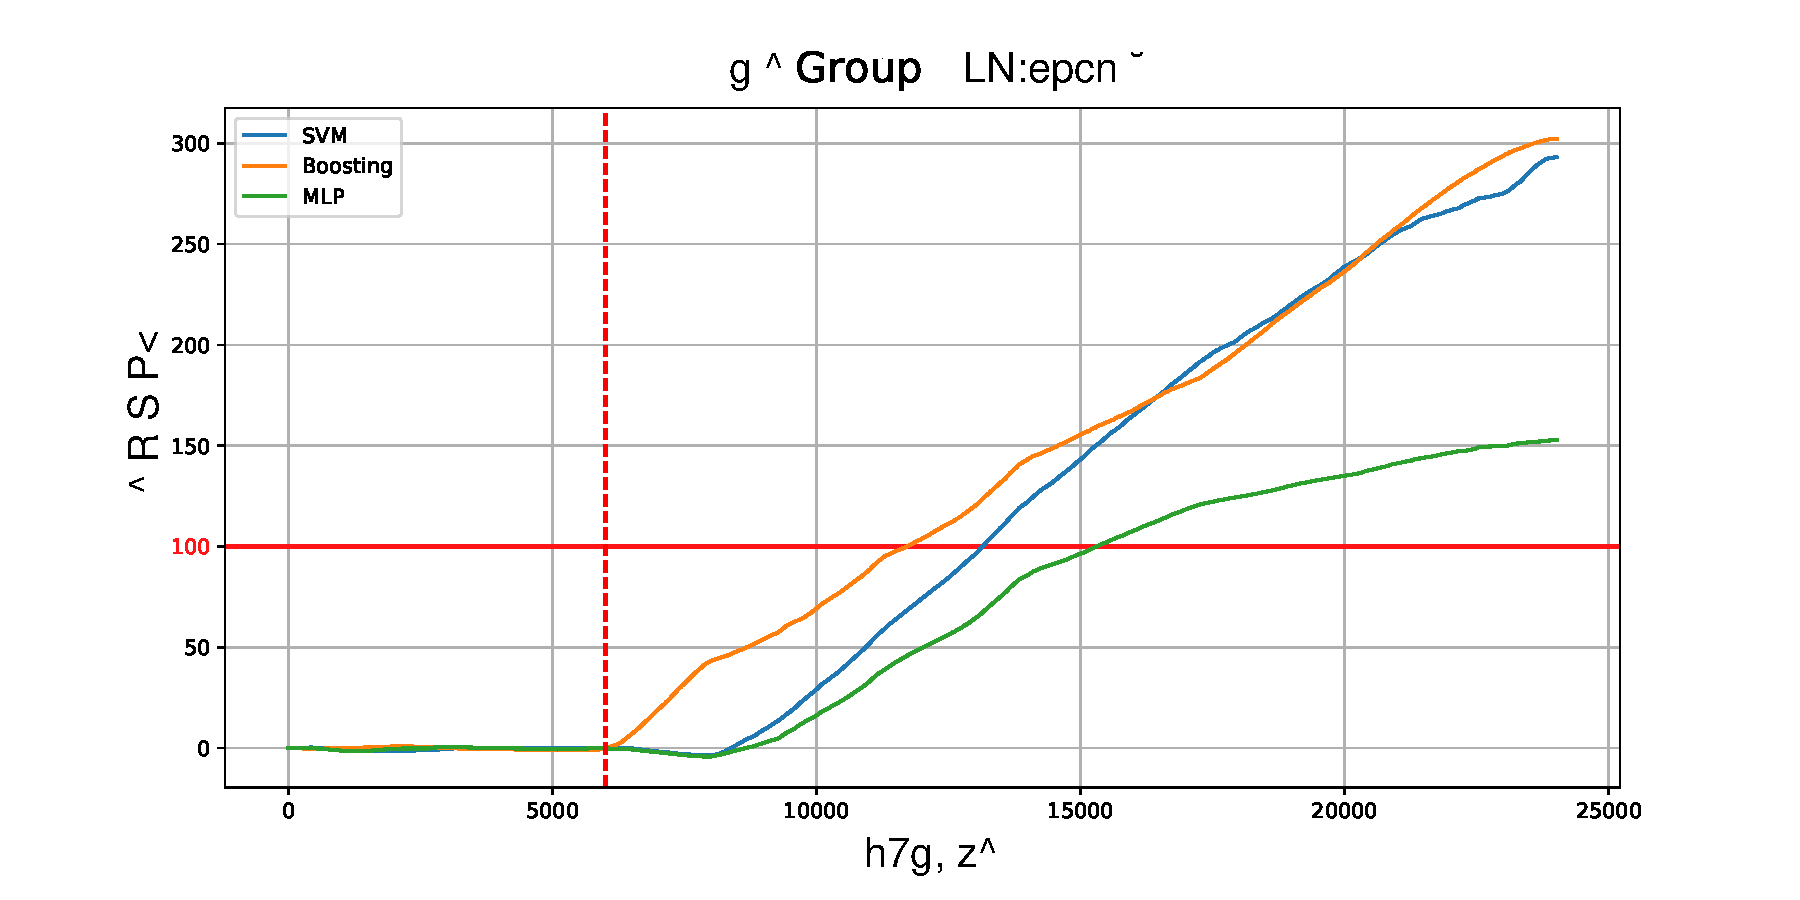
\includegraphics[width=1\linewidth]{Img/chapter9/Group data set-icml}}
\caption{{Group}行为数据集有序学习的鞅序列}
\label{fig:group-mar}
\end{figure*}
\begin{figure*}[htbp] % [tb]
\centerline{
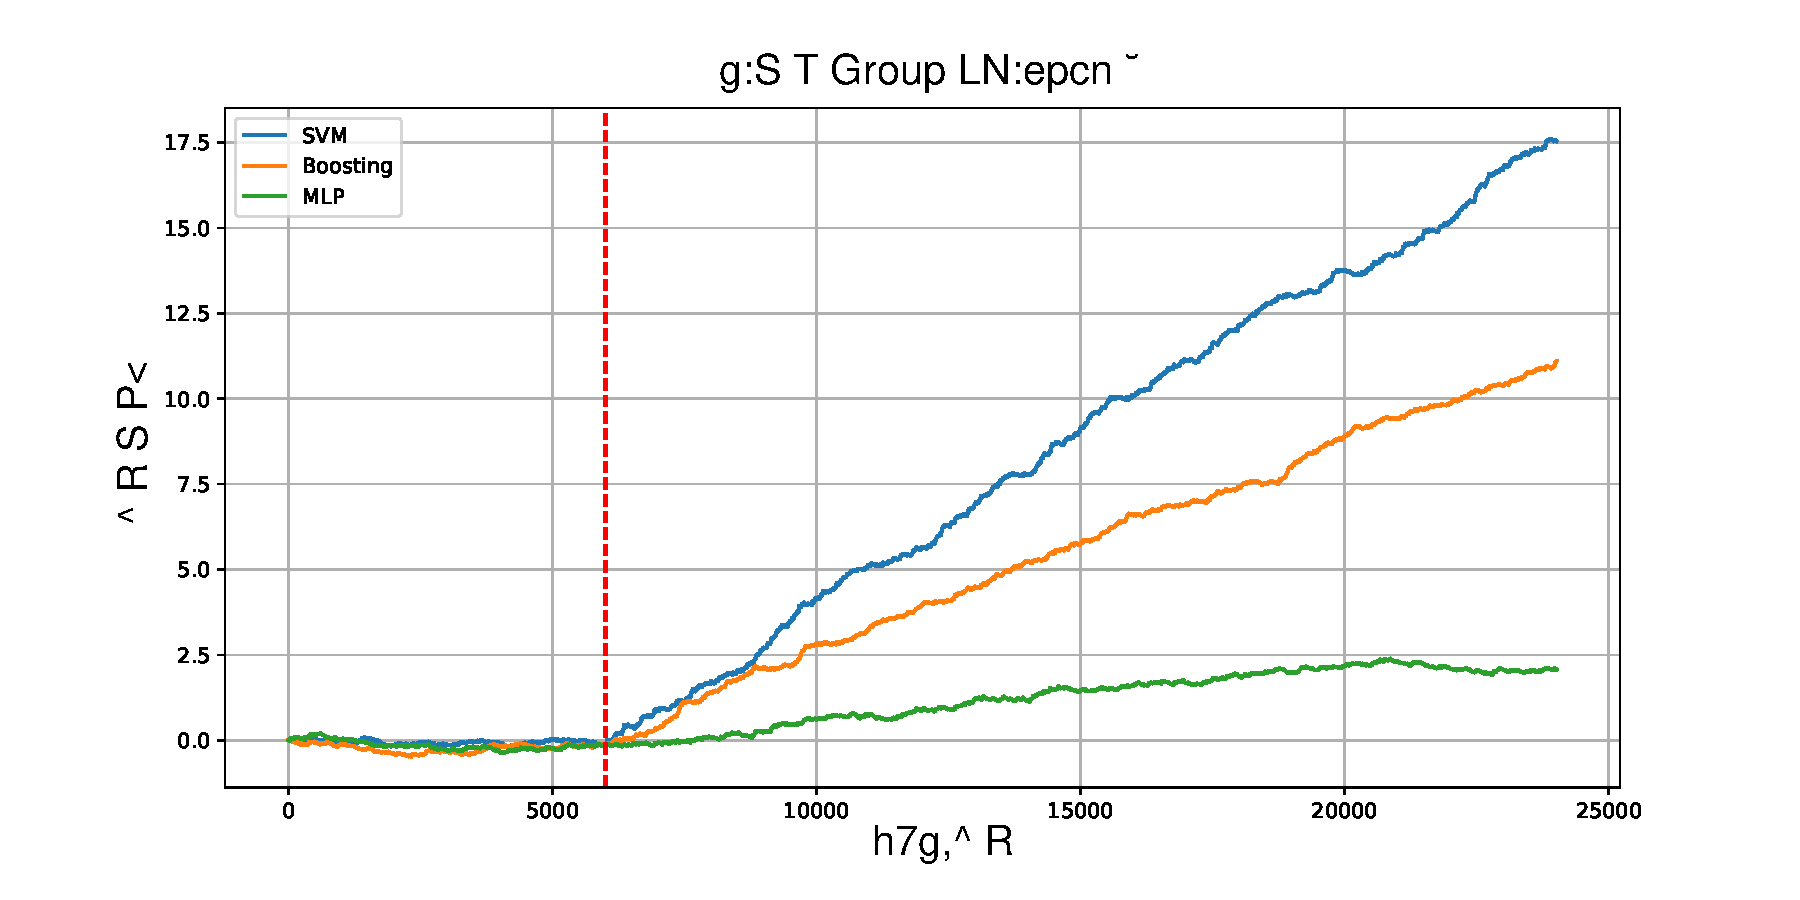
\includegraphics[width=1\linewidth]{Img/chapter9/Randomly shuffling Group data sett-icml}}
\caption{随机化{Group}行为数据集有序学习的鞅序列}
\label{fig:radom-group-mar}
\end{figure*}


\section{本章小结}
\label{sec:mar-discuss}
本章针对无人机集群行为数据的分布随着时间发生变化的特点, 结合鞅理论提出一种无分布假设的分布漂移检测方法。主要结论总结如下:
\begin{enumerate}
\item 在无人机集群数据按照本身时间顺序建模和随机采样建模两种情形下, 对比机器学习算法预测性能之间的差异。试验结果表明, 当按照数据本身顺序建模时, 机器学习算法预测错误数目远远大于随机采样情形下的预测数目;
\item 利用鞅方法检测无人机集群行为数据的分布漂移。试验结果表明, 样本数据按照本身顺序进入模型后, 鞅序列的值增长较快; 并且鞅序列取值远远大于给定阈值。根据鞅理论, 这种现象表明无人机集群行为数据发生分布漂移;
\item 对于随机采样后建模数据, 鞅序列取值虽然没有超过给定阈值, 但是鞅序列依然保持上涨的趋势。这说明对原始数据随机采样, 一方面可以获得更加高效的预测效果, 但是另一方面也说明即便是随机采样也无法消除数据本身分布漂移现象。
\end{enumerate}